\section{Groups in magnetic fields}

  \subsection{Hamiltonian transformations}
  %%%%%%%%%%%%%%%%%%%%%%%%%%
  %%%%%%%%%%%%%%%%%%%%%%%%%%
  \begin{frame}{The electronic Hamiltonian}
    \begin{itemize}
      \item<1-> For an $\gls*{gen:Ne}$-electron system in a \emphit{DarkGreen}{uniform} magnetic field $\gls*{mag:vec} = \symbf{\nabla} \times \gls*{mag:vecpot}(\gls*{bas:spatialcoord})$, consider the \emphbf{DarkGreen}{Schr\"{o}dinger--Pauli Hamiltonian} in atomic units:
      \begin{align*}
        \gls*{op:hamil}
          &= \tikzmarkin<2>[nodeStyleGreen, mark at=0.82]{kin}(0.04,-0.60)(-0.06,0.80)
            \annotate{2}{red}{(0,0)--++(0,-0.3)}{below}{%
              kinetic%
            }
            \frac{1}{2}
            \sum_{k=1}^{\gls*{gen:Ne}}
            \left\lvert
              -\hat{\symbfit{p}}_k + \gls*{mag:vecpot}(\gls*{bas:spatialcoord}[_k])
            \right\rvert^2
          \tikzmarkend{kin}
          + \tikzmarkin<3>[nodeStyleGreen, mark at=0.85]{potex}(0.04,-0.60)(-0.06,0.80)
            \annotate{3}{red}{(0,0)--++(0,-0.3)}{below}{%
              external potential%
            }
            \sum_{k=1}^{\gls*{gen:Ne}}
              \gls*{op:pot1e}[_{\symup{ext}}](\gls*{bas:spatialcoord}[_k])
          \tikzmarkend{potex}
          + \tikzmarkin<4>[nodeStyleGreen, mark at=0.82]{ee}(0.04,-0.60)(-0.06,0.80)
            \annotate{4}{red}{(0,0)--++(0,-0.3)}{below}{%
              electron--electron interaction%
            }
            \frac{1}{2}
              \sum_{k \ne l}^{\gls*{gen:Ne}}
              \frac{1}{\lvert \gls*{bas:spatialcoord}[_k] - \gls*{bas:spatialcoord}[_l] \rvert}
          \tikzmarkend{ee}
          + \tikzmarkin<5>[nodeStyleGreen, mark at=0.845]{eb}(0.04,-0.60)(-0.06,0.80)
            \annotate{5}{red}{(0,0)--++(0,-0.3)}{below}{%
              spin Zeeman interaction%
            }
              \frac{g_s}{2}
              \sum_{k=1}^{\gls*{gen:Ne}}
              \gls*{mag:vec} \cdot \hat{\symbfit{s}}_k
          \tikzmarkend{eb}
          \\[6pt]
          \onslide<6->{
            &= \tikzmarkin<7>[nodeStyleGreen, mark at=0.795]{zerofieldhamil}(0.04,-0.60)(-0.06,0.80)
              \annotate{7}{red}{(0,0)--++(0,-0.3)}{below}{%
                Zero-field Hamiltonian, $\gls*{op:hamil}[_0](\gls*{op:pot1e}[_{\symup{ext}}])$%
              }
                \frac{1}{2} \sum_{k=1}^{\gls*{gen:Ne}} \hat{p}_k^2
                + \sum_{k=1}^{\gls*{gen:Ne}}
                  \gls*{op:pot1e}[_{\symup{ext}}](\gls*{bas:spatialcoord}[_k])
                + \frac{1}{2}
                  \sum_{k \ne l}^{\gls*{gen:Ne}}
                  \frac{1}{\lvert \gls*{bas:spatialcoord}[_k] - \gls*{bas:spatialcoord}[_l] \rvert}
              \tikzmarkend{zerofieldhamil}
              + \tikzmarkin<8>[nodeStyleGreen, mark at=0.815]{linearcontrib}(0.04,-0.60)(-0.06,0.80)
                \annotate{8}{red}{(0,0)--++(0,-0.3)}{below}{%
                  Linear%
                }
                  \gls*{mag:vecpot}(\gls*{bas:spatialcoord}[_k]) \cdot \hat{\symbfit{p}}_k
                  + \frac{g_s}{2}
                  \sum_{k=1}^{\gls*{gen:Ne}}
                  \gls*{mag:vec} \cdot \hat{\symbfit{s}}_k
              \tikzmarkend{linearcontrib}
              + \tikzmarkin<8>[nodeStyleGreen, mark at=0.86]{quadcontrib}(0.04,-0.60)(-0.06,0.80)
                \annotate{8}{red}{(0,0)--++(0,-0.3)}{below}{%
                  Quadratic%
                }
                  \frac{1}{2}A^2(\gls*{bas:spatialcoord}[_k])
              \tikzmarkend{quadcontrib}
          }
          \\[6pt]
          \onslide<9->{
            &= \gls*{op:hamil}[_0](\gls*{op:pot1e}[_{\symup{ext}}])
            + \gls*{mag:vecpot}(\gls*{bas:spatialcoord}[_k]) \cdot \hat{\symbfit{p}}_k
            + \frac{g_s}{2}
            \sum_{k=1}^{\gls*{gen:Ne}}
            \gls*{mag:vec} \cdot \hat{\symbfit{s}}_k
            + \frac{1}{2}A^2(\gls*{bas:spatialcoord}[_k]).
          }
      \end{align*}

      \item<9-> How does each term transform \emphit{red}{spatially} and \emphit{blue}{temporally}?
    \end{itemize}

    \footfullcite{book:Weil2007}
    \footlessfullcite{article:Tellgren2018}
    \footlessfullcite{article:Irons2021}
  \end{frame}


  %%%%%%%%%%%%%%%%%%%%%%%%%%
  %%%%%%%%%%%%%%%%%%%%%%%%%%
  \begin{frame}[t]{Tensor transformations}
    \begin{itemize}
      \item<1-> Let $\symbfit{v}$ be a rank-$k$ Cartesian tensor in three dimensions.
      \only<2-5>{
        \item<2-> \emphit{red}{Spatially}, let $u \in \symsfup{O}(3)$ be any \emphbf{DarkGreen}{proper} or \emphbf{DarkGreen}{improper rotation} that acts on an orthogonal basis $\{\symbfit{e}_i\}$ spanning $\symbb{R}^3$ according to
        \begin{equation*}
          \hat{u}\symbfit{e}_i =
            \symbfit{e}_j
            \ \tikzmarkin<3>[nodeStyleGreen, mark at=0.84]{urep}(0.04,-0.20)(-0.06,0.40)
              \annotate{3}{red}{(0,0)--++(0,-0.3)}{below}{%
                $\symbfit{U}$: representation matrix for $u$ in $\{\symbfit{e}_i\}$%
              }
                U_{ji}
            \tikzmarkend{urep}.
        \end{equation*}
        \onslide<4->{%
          To consider the \emphit{DarkGreen}{linear} action of $u$ on $\symbfit{v}$, let $\symbfit{v}' = \hat{u}\symbfit{v}$.
          \begin{itemize}
            \item<4-> $\symbfit{v}$ is a \emphbf{red}{polar} tensor if
            \begin{equation*}
              v'_{ab\ldots k} = U_{ap} U_{bq} \ldots U_{kz}\ v_{pq\ldots z}.
            \end{equation*}
            \item<4-> $\symbfit{v}$ is an \emphbf{red}{axial} tensor if
            \begin{equation*}
              v'_{ab\ldots k} =
                \tikzmarkin<5>[nodeStyleGreen, mark at=0.83]{udet}(0.04,-0.20)(-0.06,0.40)
                  \annotate{5}{red}{(0,0)--++(0,-0.3)}{below}{%
                    $+1$ for proper rotations, $-1$ for improper rotations%
                  }
                  \lvert\symbfit{U}\rvert
                \tikzmarkend{udet}
                U_{ap} U_{bq} \ldots U_{kz}\ v_{pq\ldots z}.
            \end{equation*}
          \end{itemize}%
        }%
      }
      \only<6-7>{
        \item<6-> \emphit{blue}{Temporally}, let $\gls*{op:timerevnohat}$ be the \emphbf{DarkGreen}{time reversal} that acts on an orthogonal basis $\{\gls*{bas:spinbasis}[_1], \gls*{bas:spinbasis}[_2]\}$ of a two-component spinor according to
        \begin{equation*}
          \gls*{op:timerev}
          \begin{bmatrix}
            \gls*{bas:spinbasis}[_1] & \gls*{bas:spinbasis}[_2]
          \end{bmatrix}
          = \begin{bmatrix*}[r]
            \gls*{bas:spinbasis}[^*_2] & -\gls*{bas:spinbasis}[^*_1]
          \end{bmatrix*}.
        \end{equation*}
        \onslide<7->{%
          To consider the \emphit{DarkGreen}{antilinear} action of $\gls*{op:timerevnohat}$ on $\symbfit{v}$, let $\symbfit{v}'' = \gls*{op:timerev}\symbfit{v}$.
          \begin{itemize}
            \item<7-> $\symbfit{v}$ is a \emphbf{blue}{time-even} tensor (\emphbf{blue}{$\symbfit{i}$}-tensor) if
            \begin{equation*}
              \symbfit{v}'' = \symbfit{v}.
            \end{equation*}
            \item<7-> $\symbfit{v}$ is a \emphbf{blue}{time-odd} tensor (\emphbf{blue}{$\symbfit{c}$}-tensor) if
            \begin{equation*}
              \symbfit{v}'' = -\symbfit{v}.
            \end{equation*}
          \end{itemize}
        }%
      }
    \end{itemize}

    \footfullcite{book:Birss1966}
    \footlessfullcite{article:Bradley1968}
    \footlessfullcite{bookchapter:Lazzeretti1993}
  \end{frame}


  %%%%%%%%%%%%%%%%%%%%%%%%%%
  %%%%%%%%%%%%%%%%%%%%%%%%%%
  \begin{frame}{Tensor classifications}
    \begin{itemize}
      \item<1-> There are \emphit{DarkGreen}{four} types of tensors under spatial-temporal transformations.
      \begin{columns}[T]
        \begin{column}{.45\textwidth}
          \begin{itemize}
            \item<1-> \emphbf{red}{polar} \emphbf{blue}{time-even} tensors
            \begin{itemize}
              \item position vectors $\gls*{bas:spatialcoord}$
            \end{itemize}
          \end{itemize}
        \end{column}
        \begin{column}{.45\textwidth}
          \begin{itemize}
            \item<1-> \emphbf{red}{polar} \emphbf{blue}{time-odd} tensors
            \begin{itemize}
              \item linear momentum vectors $\symbfit{p}$
              \item magnetic vector potentials $\gls*{mag:vecpot}$
              \item current densities $\gls*{mag:jphys}$
            \end{itemize}
          \end{itemize}
        \end{column}
      \end{columns}

      \vspace{0.2cm}

      \begin{columns}[T]
        \begin{column}{.45\textwidth}
          \begin{itemize}
            \item<1-> \emphbf{red}{axial} \emphbf{blue}{time-even} tensors
          \end{itemize}
        \end{column}
        \begin{column}{.45\textwidth}
          \begin{itemize}
            \item<1-> \emphbf{red}{axial} \emphbf{blue}{time-odd} tensors
            \begin{itemize}
              \item angular momentum vectors $\symbfit{l}$
              \item magnetic field vectors $\gls*{mag:vec}$
            \end{itemize}
          \end{itemize}
        \end{column}
      \end{columns}
    \end{itemize}

    \footfullcite{book:Birss1966}
    \footlessfullcite{article:Bradley1968}
    \footlessfullcite{bookchapter:Lazzeretti1993}
  \end{frame}


  \subsection{Hamiltonian invariance}
  %%%%%%%%%%%%%%%%%%%%%%%%%%
  %%%%%%%%%%%%%%%%%%%%%%%%%%
  \begin{frame}{Symmetry and pseudo-symmetry groups}
    \begin{itemize}
      \onslide<1->{
        \begin{alertblock}{Definition (symmetry group)}
          All transformations $\hat{T}$ that leave the electronic Hamiltonian $\gls*{op:hamil}$ invariant, \ie $\hat{T}\gls*{op:hamil}\hat{T}^{-1} = \gls*{op:hamil}$, form the \emphbf{DarkGreen}{symmetry group} of $\gls*{op:hamil}$.
          Such transformations are called \emphbf{DarkGreen}{symmetry transformations}.
        \end{alertblock}
      }
      \item<1-> Symmetry transformations impose \emphit{DarkGreen}{constraints} on the eigenfunctions of $\gls*{op:hamil}$ and properties calculated from them.\\[6pt]
      \onslide<2->{
        \begin{alertblock}{Definition (pseudo-symmetry group)}
          Consider a term $\gls*{op:hamil}' \subset \gls*{op:hamil}$.
          All transformations $\hat{T}$ that leave $\gls*{op:hamil}'$ invariant but not the full $\gls*{op:hamil}$ form a \emphbf{DarkGreen}{pseudo-symmetry group} of $\gls*{op:hamil}$.
          Such transformations are called \emphbf{DarkGreen}{pseudo-symmetry transformations}.
        \end{alertblock}
      }
      \item<2-> Pseudo-symmetry transformations provide ways to understand eigenfunctions of \emphit{DarkGreen}{$\gls*{op:hamil}$ (complicated)} from the perspective of \emphit{DarkGreen}{$\gls*{op:hamil}'$ (simpler)}.
    \end{itemize}
  \end{frame}


  %%%%%%%%%%%%%%%%%%%%%%%%%%
  %%%%%%%%%%%%%%%%%%%%%%%%%%
  \begin{frame}{Groups in magnetic fields}
    \begin{itemize}
      \item<1-> Let us revisit the electronic Hamiltonian in a uniform magnetic field:
      \begin{equation*}
        \gls*{op:hamil} =
          \tikzmarkin<2-3>[nodeStyleGreen, mark at=0.79]{zerofieldhamilgroup}(0.04,-0.20)(-0.06,0.40)
            \annotate{2-3}{red, align=center}{(0,0)--++(0,-0.3)}{below}{%
              \only<2>{\emphbf{red}{polar} \emphbf{blue}{time-even}\\}%
              \only<3>{\textcolor{DarkGreen}{$\symcal{G} + \gls*{op:timerevnohat} \symcal{G}$}}%
            }
            \gls*{op:hamil}[_0](\gls*{op:pot1e}[_{\symup{ext}}])
          \tikzmarkend{zerofieldhamilgroup}
          %%%
          + \tikzmarkin<6>[nodeStyleGreen, mark at=0.83]{Apgroup}(0.04,-0.40)(-0.06,0.60)
            \annotate{6}{red, align=center}{(0,0)--++(0,-0.3)}{below}{%
              \textcolor{DarkGoldenrod}{$\symsfup{O}(3) + \gls*{op:timerevnohat} \symsfup{O}(3)$}%
            }
            \tikzmarkin<4>[nodeStyleGreen, mark at=0.82]{Agroup}(0.04,-0.20)(-0.06,0.40)
              \annotate{4}{red, align=center}{(0,0)--++(0,-0.3)}{below}{%
                \emphbf{red}{polar} \emphbf{blue}{time-odd}%
              }
              \gls*{mag:vecpot}(\gls*{bas:spatialcoord}[_k])
            \tikzmarkend{Agroup}
            \cdot
            \tikzmarkin<5>[nodeStyleGreen, mark at=0.84]{pgroup}(0.04,-0.20)(-0.06,0.40)
              \annotate{5}{red, align=center}{(0,0)--++(0,-0.3)}{below}{%
                \emphbf{red}{polar} \emphbf{blue}{time-odd}%
              }
              \hat{\symbfit{p}}_k
            \tikzmarkend{pgroup}
          \tikzmarkend{Apgroup}
          %%%
          + \tikzmarkin<7-8>[nodeStyleGreen, mark at=0.84]{Bsgroup}(0.04,-0.60)(-0.06,0.80)
            \annotate{7-8}{red, align=center}{(0,0)--++(0,-0.3)}{below}{%
              \only<7>{
                \emphbf{red}{axial} \emphbf{blue}{time-odd}%
              }%
              \only<8>{
                \textcolor{MediumVioletRed}{$\symcal{H} + \gls*{op:timerevnohat} u \symcal{H}$}\\%
                \textcolor{MediumVioletRed}{\footnotesize$(u \in \symcal{G}, \hat{u}\gls*{mag:vec} = -\gls*{mag:vec})$}%
              }
            }
            \frac{g_s}{2}
            \sum_{k=1}^{\gls*{gen:Ne}}
            \gls*{mag:vec} \cdot \hat{\symbfit{s}}_k
          \tikzmarkend{Bsgroup}
          %%%
          + \tikzmarkin<6>[nodeStyleGreen, mark at=0.84]{A2group}(0.04,-0.40)(-0.06,0.60)
            \annotate{6}{red, align=center}{(0,0)--++(0,-0.3)}{below}{%
              \textcolor{DarkGoldenrod}{$\symsfup{O}(3) + \gls*{op:timerevnohat} \symsfup{O}(3)$}%
            }
            \frac{1}{2}A^2(\gls*{bas:spatialcoord}[_k]).
          \tikzmarkend{A2group}
      \end{equation*}

      \item<10-> If $\symcal{M} = \symcal{H} + \gls*{op:timerevnohat} u \symcal{H}$ is isomorphic to a \emphbf{DarkGreen}{unitary group $\symcal{M}'$}, we write $\symcal{M} = \symcal{M}'(\symcal{H})$.
    \end{itemize}

%    \vspace{1.0cm}

    \onslide<3->{
      \begin{figure}
        \centering
        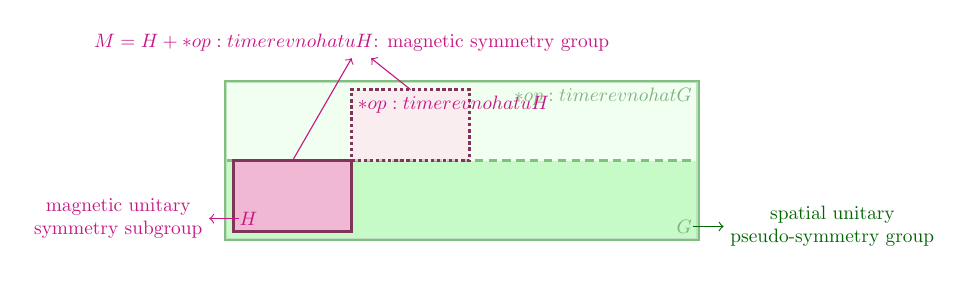
\begin{tikzpicture}
  \onslide<3->{
    \fill[fill=green!90!black, opacity=.8] (0, 0) -- (6, 0) -- (6, 1) -- (0, 1) -- cycle;
    \filldraw[fill=green!20, fill opacity=.6, draw=green!50!black, very thick] (0, 0) -- (6, 0) -- (6, 2) -- (0, 2) -- cycle;
    \draw[densely dashed, draw=green!50!black, thick] (0, 1) -- (6, 1);
    \node[anchor=south east, inner sep=3pt, scale=.7, DarkGreen] (G) at (6, 0) {$\symcal{G}$};
    \node[anchor=north east, inner sep=3pt, scale=.7, DarkGreen] at (6, 2) {$\gls*{op:timerevnohat} \symcal{G}$};
  }
  \onslide<8->{
    \filldraw[fill=white, draw=white, opacity=.5, very thick] (0, 0) -- (6, 0) -- (6, 2) -- (0, 2) -- cycle;
    \fill[fill=HotPink!90!black, opacity=.8] (0.1, 0.1) -- (1.6, 0.1) -- (1.6, 1) -- (0.1, 1) -- cycle;
    \filldraw[fill=HotPink!20, fill opacity=.6, draw=HotPink!50!black, very thick] (0.1, 0.1) -- (1.6, 0.1) -- (1.6, 1) -- (0.1, 1) -- cycle;
    \filldraw[fill=HotPink!20, fill opacity=.6, draw=HotPink!50!black, very thick, densely dotted] (1.6, 1) -- (3.1, 1) -- (3.1, 1.9) -- (1.6, 1.9) -- cycle;
    \node[anchor=south west, inner sep=3pt, scale=.7, MediumVioletRed] (H) at (0.1, 0.1) {$\symcal{H}$};
    \node[anchor=north west, inner sep=3pt, scale=.7, MediumVioletRed] at (1.6, 1.9) {$\gls*{op:timerevnohat} u \symcal{H}$};
  }
  \onslide<9->{
    \draw[->, DarkGreen, shorten <=-2] (G) -- ++(0.5, 0) node[scale=.7, anchor=west, align=center] {spatial unitary\\ pseudo-symmetry group};
    \draw[->, MediumVioletRed, shorten <=-2] (H) -- ++(-0.5, 0) node[scale=.7, anchor=east, align=center] {magnetic unitary\\ symmetry subgroup};
    \draw[->, MediumVioletRed] (0.85, 1) -- ++(0.75, 1.3) node[scale=.7, anchor=south, align=center] (maggroup) {$\symcal{M} = \symcal{H} + \gls*{op:timerevnohat} u \symcal{H}$: magnetic symmetry group};
    \draw[->, MediumVioletRed] (2.35, 1.9) -- (maggroup);
  }
\end{tikzpicture}
      \end{figure}
    }

    \footfullcite{book:Wigner1959}
    \footlessfullcite{bookchapter:Lazzeretti1993}
    \footlessfullcite{article:Keith1993}
  \end{frame}